%卒業論文用テンプレート
\documentstyle[graphicx]{jronbun}


%諸定義
\newenvironment{indention}[1]{\par
\addtolength{\leftskip}{#1}
\begingroup}{\endgroup\par}

%論文名
\title{論理回路に対する抗ノイズテストパターン生成}
%教官名
\kyoukan{高橋寛教授}
\second{王森レイ講師}
%名前
\author{~~}
%提出日
\date{平成~~年~月~日提出}
%講座名
\kouza{\gt 愛媛大学工学部情報工学科情報システム工学講座}

\begin{document}
%タイトル生成
\maketitle
%目次生成
\pagenumbering{roman}
\tableofcontents
\cleardoublepage
\pagenumbering{arabic}

%--ここから本文--
%第1章 まえがき
\chapter{まえがき}
%まえがき
本論文では、番号からラズベリーパイと各種センサとサーバを組み合わせて商品識別システムを構築した。
 皆さんもご存じの通り現在の日本は少子高齢化の流れで人的資源が減少している。総務省の調べでは総人口が2008年をピークに減少している\cite{population}.人的資源の減少という問題は私たちの身近なスーパーマーケットや小売店にも表れており、その対処法として決済の一部をユーザに一部負担してもらうセルフレジなどの導入が進んでいる。またAmazonなどの大企業では無人店舗AmazonGo\cite{amazongo}.をアメリカの一部地域で展開しているがそのサービスを稼働させるには高い技術力と資金力が必要となる。先ほど述べたセルフレジの金額も登録機と精算機を合わせて平均で300万を超えるものが多い\cite{self_register}.セルフレジの導入は人手不足問題を抱える店舗においてメリットも大きいが負担も大きい問題がある。そこでこのコスト面での問題を解決するために資金力を持たない店舗でも導入しやすい安価なシステムの構築を本研究の目的とした。

 本研究では商品の識別から決算までのシステム構築をV字モデルに従い、グループ(段原丞治、真鍋樹)で研究を行った。
要求定義や設計はUML図を用いて定義しそれをもとに開発を行う。実装に関してはエッジ処理側とサーバ処理側で担当を分けた。

 本論文は以下のような構成をとる。第2章では用語、実験環境、システム概要の説明を述べる。第3章ではUML図を用いてシステムの要求定義、設計を述べる。第4章では実装内容と検証結果を示す。第5章では実装したシステムの評価及び考察を述べる。第6章では本研究のまとめと今後の課題を示す。

%第2章 準備
\chapter{準備}
%第2章:準備
%システムを開発する際,使用した定義.


本章では,研究方針のフローと,本論文で使用する用語について述べる.

\subsection*{V字モデル[5]}

V字モデルとはソフトウェアの開発と確認の流れを模式的に示したものである.以下の図\ref{vji}にV字モデルの開発プロセスを示す.横軸は開発の時間軸であり,縦軸は詳細化の程度を表している\cite{kumikomi}.図\ref{vji}にも示すように,詳細設計は単体テスト,基本設計は結合テストによって,要求分析は総合テストによって検証する.また,逆にテスト段階で判明した不具合は,左側の対応する設計にさかのぼった作業を必要とする.本研究では開発プロセスモデルとしてV字モデルを採用した.

\begin{figure}[htbp]
\centering
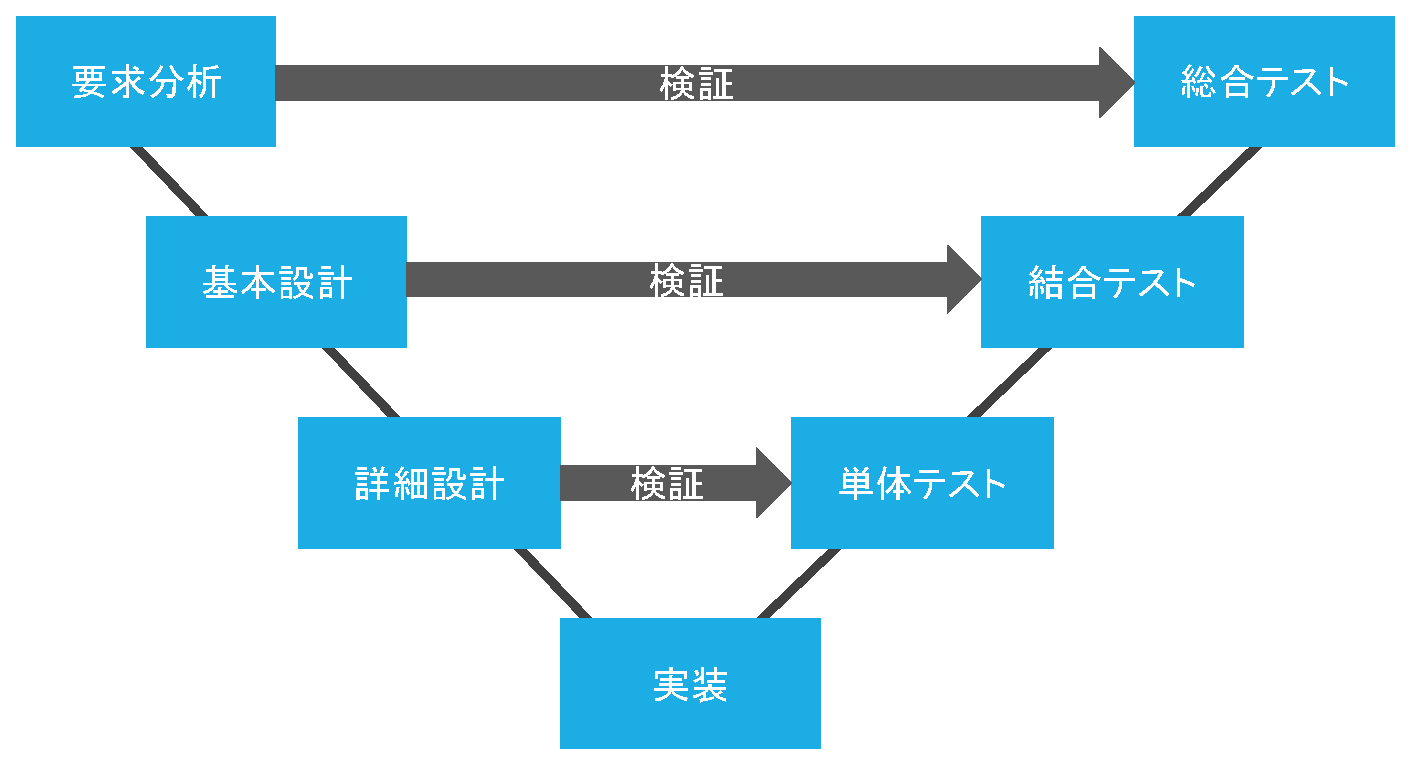
\includegraphics[width=12cm]{./picture/vjimodel.eps}
\caption{V字モデル}
\label{vji}
\end{figure}


\subsection*{UML(Unifiled Modeling Language)[3]}

UMLとは統一モデリング言語(Unified Modeling Language)のことで,ビジネスや各種システムを対象としてその構造とダイナミクス(動的な振る舞いや挙動)をわかりやすく表現するためのビジュアルな言語である\cite{uml}.UMLの導入により,下記のような効用がもたらされる.

\begin{itemize}
\item ユーザと開発者,または開発者どうしのコミュニケーションギャップの解消.
\item ユーザ要求の把握が正確になることで,仕様の認識違いによる出戻りの削減.
\item UMLによるオブジェクト指向設計が効果的にモジュール化を促進し,保守コストを削減.
\end{itemize}

\subsection*{ユースケース図[3]}

ユースケース図とは,UMLで定義されている図のうちのひとつである.ユーザの視点でシステムの機能的な流れを記述する記述法\cite{soft}であり,システムの使用イメージを表現する.システムがどのように機能すべきかという振る舞い(ユースケース)と,その外部環境(アクター)を表す.ユーザやクライアントの要求事項,システムに対して課せられている基本機能やサービス項目などの要件定義を表現するときに広く用いられる.

\subsection*{クラス図[3]}

クラス図はUMLの基本となる図のひとつである.システムをデータの視点から記述する図法\cite{soft}であり,システムが扱う情報構造を表す.問題領域の構造や対象システムの静的な構成,システムの詳細設計,あるいは企業の部門の業務モデルの基本構造,問題解決の最初のとっかかりとなる概念マップの構築,といったことに広く使うことができる.

\subsection*{シーケンス図[3]}

シーケンス図とは,UMLで定義されている相互作用図の一種類である.システムの一機能を実行の視点から記述する図法\cite{soft}	であり,システム機能がオブジェクトのメッセージのやり取りによってどのように達成されるかを示す.オブジェクト間のメッセージのやりとりを時系列に沿って並べて表現したものがシーケンス図である.

%第3章 
\chapter{抗ノイズテストパターン生成法}
%第3章
%問題解決方法の選定:表を作成して問題解決方法を比較評価する.評価の理由と根拠をあげる(要データ,関連文献)
%解決方法の実行可能性の検証:自分がこの解決方法を選択した理由を述べる(3つの観点については本参照)


本章では,まず3.1節ではスマートモビリティレジシステムの概要を述べる.3.2節ではユースケース図を用いて,スマートモビリティレジシステムの要求定義を述べる.3.3節ではクラス図を用いて,スマートモビリティレジシステムの基本設計について述べる.3.4節ではシーケンス図を用いてスマートモビリティレジシステムの詳細設計を述べる.

%第4章
\chapter{実験結果・考察}
%第4章:実験結果・考察
本章ではV字モデルにおけるて実装及び検証について述べる。ここでは具体的な実装方法について述べる。
\section{実装・実験環境}
実装はグループで行い、エッジ処理側は真鍋樹が行った。この章では筆者が担当した、サーバ側の実装についてのみ述べる。ここでは、エッジ処理側のことをクライアントと呼ぶ。実装に使用したプログラム言語は、クライアント、サーバのどちらもPython3である。


\subsection*{実験環境}
実験環境で使用したハードウェアのスペックを以下の表\ref{spec}に示す。
\begin{table}[htb]
\begin{center}
\caption{実行環境}
\begin{tabular}{|c|c|c|c|c|} \hline
処理担当 & OS & CPU & RAM & GPU \\ \hline
サーバ側 & Windows10 64bit Pro & Core2Duo E7500 2.93GHz & 4GB & GT740 \\ \hline
エッジ側 & RaspberryPi 3B(Rasbian) & Broadcom 1.2GHz & 1GB & None \\ \hline
\end{tabular}
\label{spec}
	\end{center}
\end{table}


実験環境で使用したライブラリ、プログラム言語を以下の表\ref{library_spec}に示す。
\begin{table}[htb]
\begin{center}
\caption{使用ライブラリ・使用言語}
\begin{tabular}{|c|c|c|c|c|} \hline
処理担当 & ライブラリ・使用言語名 & バージョン & 使用目的 \\ \hline \hline
サーバ側 & Python3 & 3.7.4 & メイン処理	\\ \hline
サーバ側 & OpenCV & 4.1.2 & 画像切り取り\\ \hline
サーバ側 & Yolo & 3 & バーコード領域取得\\ \hline
サーバ側 & CUDA & 10.1 & 学習に使用\\ \hline
サーバ側 & pyzbar & 0.1.8 & バーコード番号取得\\ \hline
サーバ側 & mysqlclient & 1.4.6 & DB操作\\ \hline \hline
Webページ & XAMPP & 3.2.4 & Webページ、DBホスト\\ \hline
Webページ & apache2 & 2.4.41 & Webページホスト\\ \hline
Webページ & MariaDB & 10.4.10 & DB\\ \hline
Webページ & PHP & 7.3.12 & Webページ処理、DB操作\\ \hline \hline
エッジ側 & Python3 & 3.7.3 & メイン処理		\\ \hline
エッジ側 & OpenCV & 3.4.3 & Webカメラ操作\\ \hline
\end{tabular}
\label{library_spec}
	\end{center}
\end{table}


\newpage

\subsection*{サーバ通信}
クライアントとのデータのやり取りを含めた連携には、通信処理が必要不可欠になる。クライアントは、距離センサの反応後、カメラを起動し複数の画像を撮影する。クライアントからサーバへ送信するデータは、画像データとフラグをセットしたものである。しかしながら、ソケット通信において送信処理が複数回であったとしても、受信処理ではひとまとまりのデータとして受け取られることがある。その問題を防ぐために、送信データのヘッダにデータのサイズを書き込む手段をとった。
クライアントから送られてきた画像データはバイナリ形式になっているので、OpenCV\cite{opencv}のフォーマットに変換する。

\subsection*{Yoloによるバーコード領域特定}
Yoloを使用した理由は、pyzbar\cite{pyzbar}の識別精度にある問題があったからである。pyzbar\cite{pyzbar}は、近距離で撮影したバーコードの画像の認識はできるが、距離が離れると識別しなくなる。これは、画像の中に占めるバーコード部分が少なくなることが原因であると考えられる。そこで、Yoloを使用し画像からバーコードの部分の座標を取得する。画像のうち、バーコードの部分のみをpyzbarに渡すことで、距離が離れていても近距離で撮影したのと同じ効果が得られるようになった。学習には、バーコードの画像を約2000枚用意した。Yoloの実行はサーバ側で行う。当初、クライアント側であるRaspberryPiでYoloを実行すればサーバは不要になり、通信におけるタイムラグもなくなることが仮定された。ところが、RaspberryPiの性能ではYoloを、高い識別精度を保ったままリアルタイムに動作させることは、性能上難しいと判断したためサーバで行うことになった。

\newpage

\subsection*{DBを使用した商品情報の管理}
カゴの中の商品の管理と、商品自体の情報の管理のために、DBを使用した。本研究ではMariaDBを使用した。カゴDBの構造を以下に示す。
始めに、商品自体のデータを管理するitemテーブルを表\ref{item_db}に示す。janとはJANコードのことであり、商品識別番号である。titleは、商品名のことである。priceは、商品の価格を示す。
image\_urlは、商品の画像があるURLを示している。最後の、image\_rawはこのシステムでは使用していないが、画像データそのものを格納する。
\begin{table}[htbp]
\centering
\caption{itemテーブル}
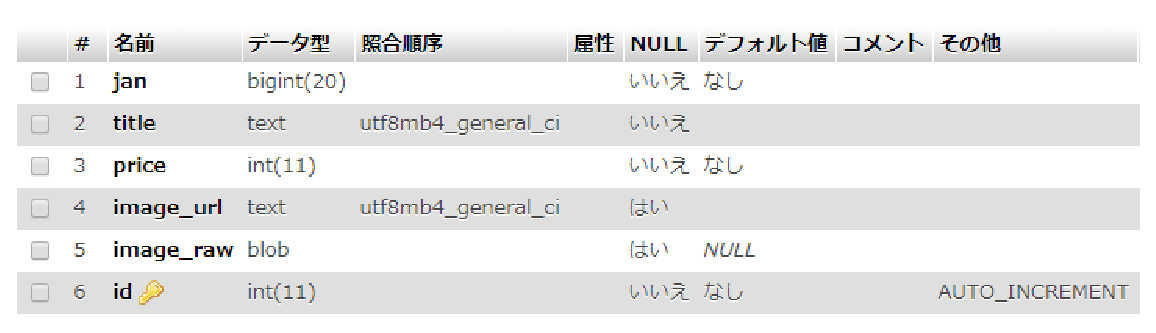
\includegraphics[width=15cm]{./pic/item_db.eps}
\label{item_db}
\end{table}

\newpage

次に、cartテーブルの構造を表\ref{cart_db}に示す。idは、テーブルのレコードの固有番号を示すためにある。janは、JANコードのことである。cart\_idはカートの固有番号を示す。この番号でカートごとの区別を行う。この番号があることで複数カートを運用した際も区別することができる。
%%%商品DB
\begin{table}[htbp]
\centering
\caption{cartテーブル}
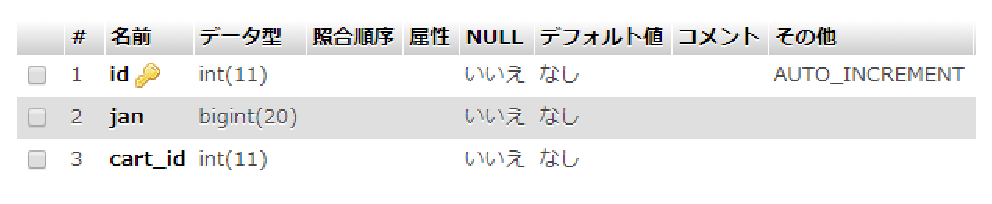
\includegraphics[width=15cm]{./pic/cart_db.eps}
\label{cart_db}
\end{table}


customerテーブルの構造を表\ref{customer_db}に示す。このcustomerテーブルは、顧客情報を管理する。idは顧客の固有番号を示す。balanceは、顧客の所持金額を示す。

\begin{table}[htbp]
\centering
\caption{customerテーブル}
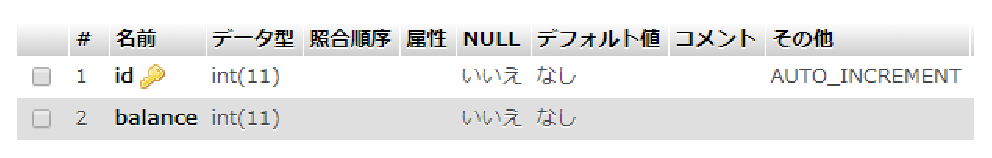
\includegraphics[width=15cm]{./pic/customer.eps}
\label{customer_db}
\end{table}

\newpage

\subsection*{決済システム}
設計段階では、決済システムの動作は、ユーザが退店する際に自動で行われる。しかし、その機能を実装するには時間の都合上難しいと判断したため、仮の決済用のWebページを作成してテストを行っている。Webページ作成にはPHPとHtmlを使用した。以下にWebページの動作の手順を示す。

\subsection*{カート画面}
以下の図\ref{web_cart}は、どのカートを使用するか選択するためにある。
\begin{figure}[htbp]
\centering
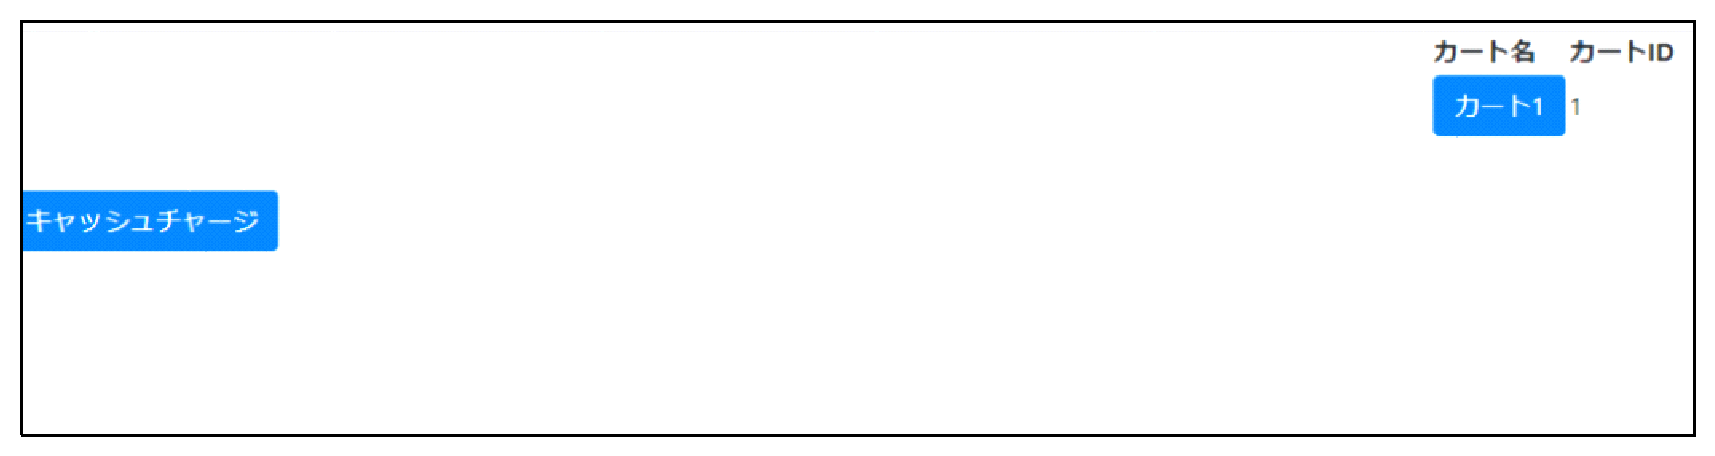
\includegraphics[width=15cm]{./pic/web/1.eps}
\caption{Webページ カート画面}
\label{web_cart}
\end{figure}

\subsection*{カート内商品一覧}
図\ref{web_cart_items}は、カート内にある購入予定商品の一覧を表している。表示内容は、商品名と価格、商品画像、個数の4つである。ページ内にある緑のボタンを押すと、会計が行われる。
\begin{figure}[htbp]
\centering
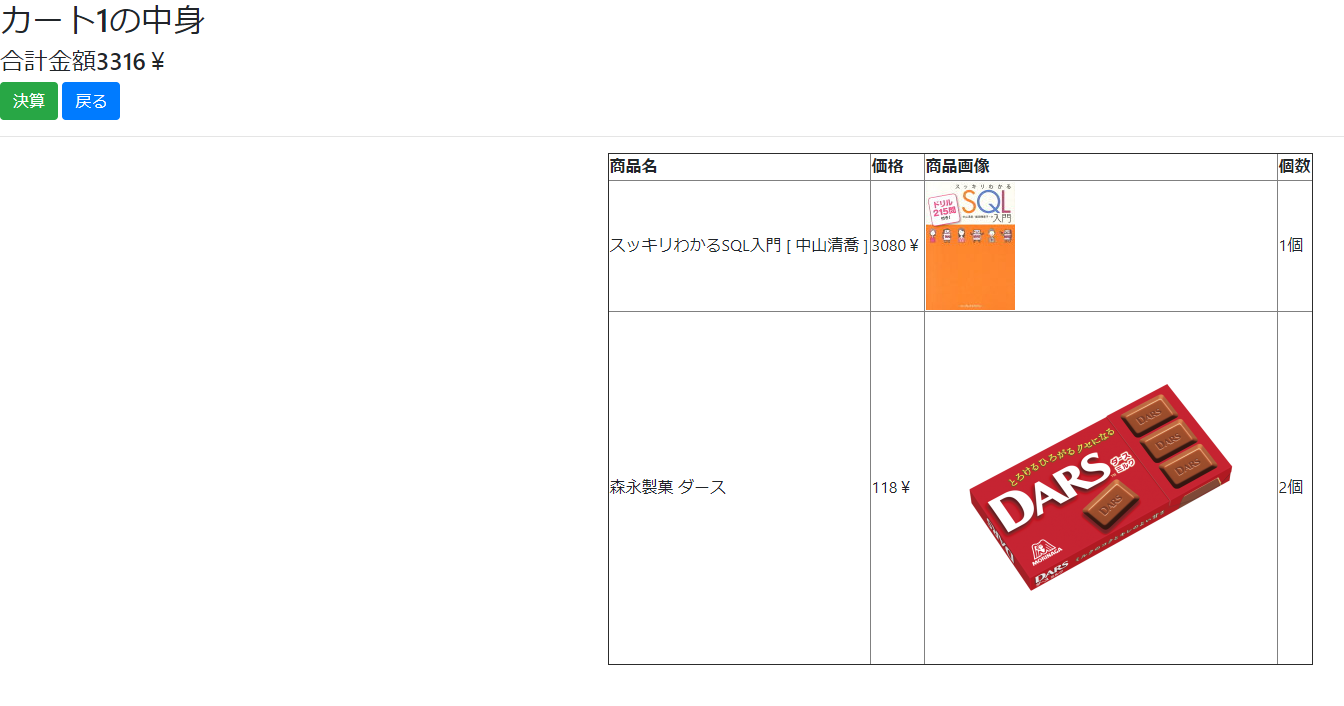
\includegraphics[width=15cm]{./pic/web/2.eps}
\caption{Webページ カート内商品一覧}
\label{web_cart_items}
\end{figure}

\subsection*{決済完了画面}
図\ref{web_cart_items}のページで緑のボタンを押すと、図\ref{web_checksum}画面に移行する。移行後は図\ref{web_checksum}のとおりに顧客の所持金から購入金額が差し引かれ、残高が表示される。また、所持金が購入金額が下回っていた場合は、所持金額が足りないと警告され決済は行われない。
\begin{figure}[htbp]
\centering
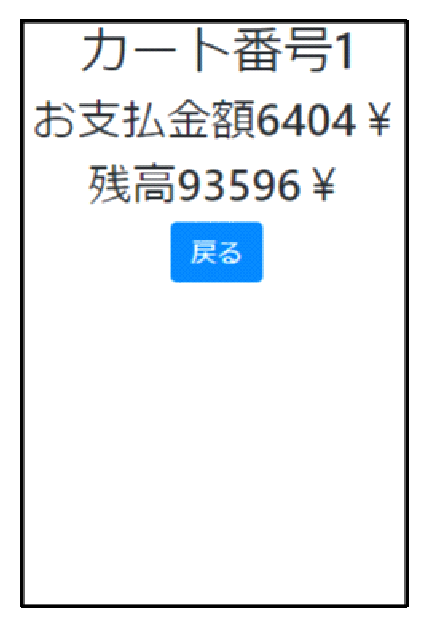
\includegraphics[width=10cm,height=10cm]{./pic/web/3.eps}
\caption{Webページ 決済完了}
\label{web_checksum}
\end{figure}

\newpage

%第5章
\chapter{あとがき}
%あとがき


%--ここまで本文--


%謝辞
\newpage
\addcontentsline{toc}{chapter}{\protect\numberline{謝辞}{}}
\chapter*{謝辞}
%--ここから謝辞--
本研究を進めるにあたり,懇篤な御指導,御鞭撻を賜わりました本学高橋寛教授に深く御礼申し上げます.

本論文の作成に関し,詳細なるご検討,貴重な御教示を頂きました本学樋上喜信准教授に深く御礼申し上げます.

また,審査頂いた本学岡野大准教授ならびに宇戸寿幸准教授に深く御礼申し上げます.

最後に,多大な御協力と貴重な御助言を頂いた本学工学部情報工学科情報システム工学講座高橋研究室の諸氏に厚く御礼申し上げます.

%--ここまで謝辞--

%参考文献
\begin{thebibliography}{99}
%ここから参考文献

%--例--
\bibitem{Interconnect}
Bram Kruseman , Ananta K. Majihi , Wilmar Heuvalman , Jennifer Dworak“NIM-X : A Noise Index Model-Based X-Filling technique to Overcome the Power Supply Switching Noise Effects on Path Delay Test" IEEE Trans. on VLSI Test Symp. ,pp.809-813, May. 2012.
%ここまで参考文献

\end{thebibliography}
\end{document}
